\documentclass{article}
\usepackage{amsmath}
\usepackage{tikz}
\begin{document}

Given: \
Initial Velocity = $100 \frac{\text{km}}{\text{h}} [\text{NW}]$ \
Final Velocity = $50 \frac{\text{km}}{\text{h}} [\text{E}]$ \
Time to change direction = $4$ seconds \

We can find the change in velocity by subtracting the initial velocity from the final velocity:

\begin{align*}
\Delta \vec{v} &= \vec{v}_f - \vec{v}_i \
&= 50 \frac{\text{km}}{\text{h}} [\text{E}] - 100 \frac{\text{km}}{\text{h}} \left[\frac{1}{\sqrt{2}},\frac{1}{\sqrt{2}}\right] \
&= \sqrt{5000} \frac{\text{km}}{\text{h}} [\text{N}60^\circ\text{E}]
\end{align*}

The velocity vector in km/h is converted to m/s using the conversion factor of $1$ km/h $= 0.2777778$ m/s:

\begin{align*}
\Delta \vec{v} &= \sqrt{5000} \frac{\text{km}}{\text{h}} [\text{N}60^\circ\text{E}] \times \frac{1000}{3600} \frac{\text{m}}{\text{s}\cdot \text{km}} \
&= \frac{50}{3} \frac{\text{m}}{\text{s}} [\text{N}60^\circ\text{E}]
\end{align*}

The average acceleration is then calculated as:

\begin{align*}
\vec{a}_{avg} &= \frac{\Delta \vec{v}}{\Delta t} \
&= \frac{50}{3} \frac{\text{m}}{\text{s}} [\text{N}60^\circ\text{E}] \div 4 \text{ s} \
&= 9.72 \frac{\text{m}}{\text{s}^2} [\text{E}30^\circ\text{S}]
\end{align*}

Therefore, the average acceleration is $9.72$ m/s$^2$ [E30S].

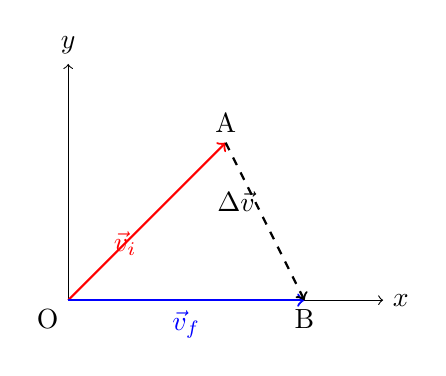
\begin{tikzpicture}
  % Draw x and y axes with labels
  \draw[->] (0,0) -- (4,0) node[right] {$x$};
  \draw[->] (0,0) -- (0,3) node[above] {$y$};
  \coordinate (start) at (0,0);
  \coordinate (initial) at (2,2);
  \draw[->, thick, red] (start) -- (initial) node[midway, below left] {$\vec{v}_i$};
  \coordinate (end) at (4,0);
  \coordinate (final) at (3,0);
  \draw[->, thick, blue] (start) -- (final) node[midway, below] {$\vec{v}_f$};
  \draw[dashed, ->, thick] (initial) -- (final) node[midway, above left] {$\Delta \vec{v}$};
  \draw (0,0) node[below left] {O};
  \draw (initial) node[above] {A};
  \draw (final) node[below] {B};
\end{tikzpicture}  

\end{document}
